\documentclass[11pt]{article}

%% -- LaTeX packages --
\usepackage[utf8]{inputenc}
\usepackage[T1]{fontenc}
\usepackage{lmodern}
\usepackage{amsmath,amssymb}
\usepackage{graphicx}
\usepackage{booktabs}
\usepackage{algorithm}
\usepackage{algpseudocode}
\usepackage{hyperref}
\usepackage{natbib}
\usepackage[margin=1in]{geometry}
\usepackage{xcolor}
\usepackage{listings}

%% Custom commands for JSS-style markup
\newcommand{\proglang}[1]{\textsf{#1}}
\newcommand{\pkg}[1]{\textbf{#1}}
\newcommand{\code}[1]{\texttt{#1}}
\newcommand{\fct}[1]{\code{#1()}}
\newcommand{\class}[1]{`\code{#1}'}

%% Listings settings for R code
\lstset{
  language=R,
  basicstyle=\ttfamily\small,
  breaklines=true,
  showstringspaces=false,
  backgroundcolor=\color{gray!10},
  frame=single,
  framerule=0pt,
  xleftmargin=10pt,
  xrightmargin=10pt,
  aboveskip=10pt,
  belowskip=10pt
}

%% Title and authors
\title{\pkg{RcppML}: High-Performance Non-Negative Matrix Factorization\\
with Cross-Validation for \proglang{R}}

\author{Zachary DeBruine\\
Department of Computational Medicine and Bioinformatics\\
University of Michigan\\
\texttt{debruine@umich.edu}}

\date{}

\begin{document}

\maketitle

\begin{abstract}
Non-negative matrix factorization (NMF) is a fundamental dimensionality 
reduction technique with applications spanning bioinformatics, text mining, 
computer vision, and signal processing. This paper presents \pkg{RcppML}, an 
\proglang{R} package that implements a comprehensive NMF framework with several 
key innovations: (1) a highly optimized sequential coordinate descent solver for 
non-negative least squares with support for L1 regularization and bounded 
solutions; (2) streaming cross-validation with minimal computational overhead 
using a novel position-dependent random number generator; (3) multiple robust 
loss functions including MSE, MAE, Huber, and KL-divergence implemented via 
iteratively reweighted least squares; (4) automatic rank determination through 
golden section search optimization; (5) specialized rank-2 NMF for 
high-performance spectral bipartitioning. The package provides unified support 
for both sparse and dense matrices through template metaprogramming and achieves 
state-of-the-art performance through careful cache-aware algorithm design. We 
demonstrate that \pkg{RcppML} outperforms existing implementations while 
providing principled model selection through integrated cross-validation.

\vspace{1em}
\noindent\textbf{Keywords:} non-negative matrix factorization, cross-validation, coordinate 
descent, spectral clustering, \proglang{R}, \proglang{C++}, \pkg{Rcpp}
\end{abstract}


%% =============================================================================
\section{Introduction} \label{sec:introduction}

Non-negative matrix factorization (NMF) decomposes a non-negative matrix 
$\mathbf{A} \in \mathbb{R}_{\geq 0}^{m \times n}$ into two non-negative factor 
matrices $\mathbf{W} \in \mathbb{R}_{\geq 0}^{m \times k}$ and 
$\mathbf{H} \in \mathbb{R}_{\geq 0}^{k \times n}$ such that 
$\mathbf{A} \approx \mathbf{W}\mathbf{H}$ \citep{Lee1999}. The non-negativity 
constraints enable parts-based, interpretable representations that have proven 
valuable across diverse domains including facial recognition \citep{Lee1999}, 
text mining \citep{Xu2003}, gene expression analysis \citep{Brunet2004}, and 
single-cell genomics \citep{Kotliar2019}.

Despite its widespread use, practical NMF deployment faces several challenges. 
First, selecting the factorization rank $k$ is critical but often performed 
heuristically or through computationally expensive techniques like consensus 
clustering \citep{Brunet2004}. Second, NMF optimization is sensitive to outliers 
when using standard squared error loss. Third, achieving high performance 
requires careful algorithm engineering, particularly for sparse data common in 
modern applications.

The \pkg{RcppML} package for \proglang{R} addresses these challenges through 
several key contributions:

\begin{enumerate}
  \item \textbf{Integrated cross-validation}: A streaming algorithm that 
  computes held-out reconstruction error with minimal overhead ($<$5\% typical), 
  enabling principled rank selection without external validation frameworks.
  
  \item \textbf{Robust loss functions}: Support for MSE, MAE, Huber, and 
  KL-divergence losses implemented via iteratively reweighted least squares 
  (IRLS), providing robustness to outliers and flexibility for different data 
  types.
  
  \item \textbf{Automatic rank determination}: Golden section search 
  optimization over the cross-validation objective to automatically identify 
  optimal rank.
  
  \item \textbf{Specialized rank-2 NMF}: A highly optimized implementation for 
  spectral bipartitioning that outperforms truncated SVD approaches.
  
  \item \textbf{High-performance implementation}: Cache-aware sequential 
  coordinate descent with unified support for sparse and dense matrices through 
  \proglang{C++} template metaprogramming.
\end{enumerate}

The package is implemented as a header-only \proglang{C++} library integrated 
with \proglang{R} through \pkg{Rcpp} \citep{Eddelbuettel2011, Eddelbuettel2013}. 
All core algorithms are expressed generically over sparse 
(\class{dgCMatrix}) and dense (\class{matrix}) inputs, achieving optimal 
performance for each storage format without code duplication.

This paper is organized as follows. Section~\ref{sec:algorithm} describes the 
NMF algorithm including the coordinate descent solver and diagonal scaling 
formulation. Section~\ref{sec:crossvalidation} presents the cross-validation 
framework with streaming loss accumulation. Section~\ref{sec:lossfunctions} 
details the supported loss functions and IRLS implementation. 
Section~\ref{sec:automatic} describes automatic rank determination. 
Section~\ref{sec:bipartition} presents the rank-2 NMF specialization for 
spectral clustering. Section~\ref{sec:implementation} discusses implementation 
details and performance considerations. Section~\ref{sec:illustrations} provides 
worked examples, and Section~\ref{sec:summary} concludes.


%% =============================================================================
\section{NMF algorithm} \label{sec:algorithm}

\subsection{Problem formulation}

We formulate NMF with a scaling diagonal that separates factor magnitude from 
factor direction. Given $\mathbf{A} \in \mathbb{R}_{\geq 0}^{m \times n}$, we 
seek:
\begin{equation}
  \min_{\mathbf{W}, \mathbf{D}, \mathbf{H}} 
  \mathcal{L}(\mathbf{A}, \mathbf{W}\mathbf{D}\mathbf{H}) + 
  \lambda_1 \|\mathbf{W}\|_1 + \lambda_1 \|\mathbf{H}\|_1
  \label{eq:objective}
\end{equation}
subject to $\mathbf{W}, \mathbf{H} \geq 0$, $\mathbf{D} = \text{diag}(d_1, 
\ldots, d_k)$, and optional column normalization $\|\mathbf{w}_j\|_2 = 1$ for 
$j = 1, \ldots, k$.

The diagonal scaling $\mathbf{D}$ provides several benefits: (1) it decouples 
factor magnitude from direction, improving convergence; (2) it enables 
consistent comparison across runs with different initializations; (3) it 
facilitates L1 regularization by normalizing factor scales.

\subsection{Alternating least squares}

We optimize Equation~\ref{eq:objective} using alternating least squares (ALS), 
iteratively solving:
\begin{align}
  \mathbf{H} &\leftarrow \arg\min_{\mathbf{H} \geq 0} 
  \|\mathbf{A} - \mathbf{W}\mathbf{D}\mathbf{H}\|_F^2 + \lambda_1\|\mathbf{H}\|_1 
  \label{eq:h_update} \\
  \mathbf{W} &\leftarrow \arg\min_{\mathbf{W} \geq 0} 
  \|\mathbf{A}^\top - \mathbf{H}^\top\mathbf{D}\mathbf{W}^\top\|_F^2 + 
  \lambda_1\|\mathbf{W}\|_1
  \label{eq:w_update}
\end{align}

Each subproblem decomposes into independent non-negative least squares (NNLS) 
problems over columns. For the $\mathbf{H}$ update, letting 
$\tilde{\mathbf{W}} = \mathbf{W}\mathbf{D}$, we solve for each column $j$:
\begin{equation}
  \mathbf{h}_j \leftarrow \arg\min_{\mathbf{h} \geq 0} 
  \|\mathbf{a}_j - \tilde{\mathbf{W}}\mathbf{h}\|_2^2 + \lambda_1\|\mathbf{h}\|_1
  \label{eq:nnls}
\end{equation}

\subsection{Sequential coordinate descent solver}

We solve Equation~\ref{eq:nnls} using sequential coordinate descent 
\citep{Franc2005}. The algorithm iteratively updates each coordinate while 
holding others fixed:
\begin{equation}
  h_i \leftarrow \max\left(0, \frac{\mathbf{w}_i^\top(\mathbf{a} - 
  \tilde{\mathbf{W}}\mathbf{h}) + h_i \|\mathbf{w}_i\|_2^2 - \lambda_1}
  {\|\mathbf{w}_i\|_2^2}\right)
  \label{eq:cd_update}
\end{equation}

The key insight is to maintain the residual $\mathbf{r} = \mathbf{a} - 
\tilde{\mathbf{W}}\mathbf{h}$ incrementally. After updating $h_i$ to 
$h_i^{\text{new}}$, we update:
\begin{equation}
  \mathbf{r} \leftarrow \mathbf{r} - (h_i^{\text{new}} - h_i)\mathbf{w}_i
  \label{eq:residual_update}
\end{equation}

This reduces the complexity of each coordinate update from $O(mk)$ to $O(m)$, 
making the overall NNLS solve $O(mk)$ per column.

Algorithm~\ref{alg:cd_nnls} presents the complete coordinate descent NNLS 
solver. The inner loop terminates when no coordinate changes significantly, 
typically requiring only 2--5 passes for well-conditioned problems.

\begin{algorithm}[t]
\caption{Coordinate descent NNLS with L1 regularization}
\label{alg:cd_nnls}
\begin{algorithmic}[1]
\Require Target $\mathbf{a}$, basis $\tilde{\mathbf{W}}$, L1 penalty $\lambda_1$, 
tolerance $\varepsilon$
\State $\mathbf{h} \leftarrow \mathbf{0}$; $\mathbf{r} \leftarrow \mathbf{a}$; 
$\mathbf{g} \leftarrow \text{diag}(\tilde{\mathbf{W}}^\top\tilde{\mathbf{W}})$
\Repeat
  \State $\text{max\_update} \leftarrow 0$
  \For{$i = 1, \ldots, k$}
    \State $h_i^{\text{old}} \leftarrow h_i$
    \State $h_i \leftarrow \max\left(0, \frac{\mathbf{w}_i^\top\mathbf{r} + 
    h_i g_i - \lambda_1}{g_i}\right)$
    \If{$h_i \neq h_i^{\text{old}}$}
      \State $\mathbf{r} \leftarrow \mathbf{r} - (h_i - h_i^{\text{old}})
      \mathbf{w}_i$
      \State $\text{max\_update} \leftarrow \max(\text{max\_update}, 
      |h_i - h_i^{\text{old}}|)$
    \EndIf
  \EndFor
\Until{$\text{max\_update} < \varepsilon$}
\State \Return $\mathbf{h}$, $\mathbf{r}$
\end{algorithmic}
\end{algorithm}

\subsection{Diagonal scaling}

After each ALS iteration, we update the diagonal scaling:
\begin{equation}
  d_i \leftarrow d_i \cdot \|\mathbf{w}_i\|_2, \quad 
  \mathbf{w}_i \leftarrow \frac{\mathbf{w}_i}{\|\mathbf{w}_i\|_2}
  \label{eq:scaling}
\end{equation}

This maintains $\|\mathbf{w}_i\|_2 = 1$ throughout optimization while 
accumulating magnitude in $\mathbf{D}$. The scaling is applied after each 
$\mathbf{W}$ update and before the subsequent $\mathbf{H}$ update.


%% =============================================================================
\section{Cross-validation framework} \label{sec:crossvalidation}

\subsection{Motivation}

Selecting the factorization rank $k$ is a fundamental challenge in NMF. Common 
approaches include examining reconstruction error curves for ``elbows,'' 
computing cophenetic correlation from consensus clustering \citep{Brunet2004}, 
or using information criteria. These methods are either subjective, 
computationally expensive, or rely on asymptotic assumptions that may not hold.

Cross-validation provides a principled alternative: hold out a random subset of 
entries, fit NMF on the observed entries, and evaluate reconstruction error on 
the held-out entries. The optimal rank minimizes held-out error, directly 
measuring predictive performance rather than relying on heuristics.

\subsection{Zero-masking for sparse matrices}

For cross-validation in NMF, we mask a random fraction of non-zero entries by 
setting them to zero during fitting. The key insight is that for sparse data, 
we only mask non-zeros---zeros are uninformative since NMF naturally predicts 
small values for unobserved entries.

Let $\Omega$ denote the set of observed (non-zero) entries and 
$\Omega_{\text{test}} \subset \Omega$ denote the held-out test set. We fit NMF 
on $\mathbf{A}_{\text{train}}$ where:
\begin{equation}
  [\mathbf{A}_{\text{train}}]_{ij} = \begin{cases}
    0 & \text{if } (i,j) \in \Omega_{\text{test}} \\
    A_{ij} & \text{otherwise}
  \end{cases}
  \label{eq:masking}
\end{equation}

The test error is then computed as:
\begin{equation}
  \text{MSE}_{\text{test}} = \frac{1}{|\Omega_{\text{test}}|} 
  \sum_{(i,j) \in \Omega_{\text{test}}} (A_{ij} - [\mathbf{W}\mathbf{D}
  \mathbf{H}]_{ij})^2
  \label{eq:test_mse}
\end{equation}

\subsection{Position-dependent random masking}

A na\"ive implementation would require: (1) generating and storing the mask 
$\Omega_{\text{test}}$; (2) creating the masked training matrix; (3) iterating 
over test entries to compute error. This imposes significant memory and 
computational overhead.

Instead, we use a position-dependent random number generator that deterministically 
determines whether each entry is masked based on its position $(i, j)$:
\begin{equation}
  \text{mask}(i, j) = \mathbf{1}[\text{hash}(i, j, \text{seed}) < p_{\text{cv}}]
  \label{eq:speckled}
\end{equation}

We implement this using a variant of the PCG (Permuted Congruential Generator) 
family \citep{ONeill2014} that mixes row index, column index, and a global seed:
\begin{align}
  \text{state} &= i \oplus (j \ll 16) \oplus \text{seed} \\
  \text{state} &= \text{state} \cdot 6364136223846793005 + 1442695040888963407 \\
  \text{output} &= ((\text{state} \gg 22) \oplus \text{state}) \gg 
  (22 + (\text{state} \gg 61))
  \label{eq:pcg}
\end{align}

This ``speckled'' RNG has several advantages: (1) no memory allocation for the 
mask; (2) the same entry maps to the same mask value throughout optimization; 
(3) parallel evaluation across entries; (4) reproducibility through the seed.

\subsection{Streaming loss accumulation}

During each ALS iteration, we accumulate test error ``for free'' within the 
NNLS solve. Recall that the coordinate descent solver maintains the residual 
$\mathbf{r} = \mathbf{a} - \tilde{\mathbf{W}}\mathbf{h}$. For the $j$-th column:
\begin{equation}
  \text{test\_mse}_j = \sum_{\{i : \text{mask}(i,j)=1\}} r_i^2
  \label{eq:streaming}
\end{equation}

The total test MSE is accumulated across all columns:
\begin{equation}
  \text{MSE}_{\text{test}} = \frac{1}{|\Omega_{\text{test}}|} 
  \sum_{j=1}^{n} \text{test\_mse}_j
  \label{eq:total_test}
\end{equation}

This streaming approach has $O(1)$ memory overhead and minimal computational 
overhead, as we simply check the mask and accumulate squared residuals during 
the normal NNLS computation.

\subsection{Overhead analysis}

The cross-validation overhead comes from three sources:
\begin{enumerate}
  \item \textbf{Mask evaluation}: One RNG call per non-zero entry per column 
  solve, $O(\text{nnz})$ operations.
  \item \textbf{Loss accumulation}: One conditional addition per non-zero entry, 
  $O(\text{nnz})$ operations.
  \item \textbf{Reduced fitting signal}: Masked entries contribute zeros instead 
  of true values, potentially requiring more iterations.
\end{enumerate}

In practice, the first two sources contribute $<$5\% overhead for typical sparse 
matrices. The third source depends on the CV fraction; with 10\% masking, 
convergence is typically unaffected.


%% =============================================================================
\section{Loss functions} \label{sec:lossfunctions}

\subsection{Iteratively reweighted least squares}

The coordinate descent solver naturally handles squared error loss. To support 
alternative losses, we use iteratively reweighted least squares (IRLS), which 
reduces robust regression to a sequence of weighted least squares problems.

For a general loss $\rho(r)$, the weighted least squares formulation uses 
weights:
\begin{equation}
  w(r) = \frac{\rho'(r)}{r}
  \label{eq:irls_weights}
\end{equation}

The coordinate descent update becomes:
\begin{equation}
  h_i \leftarrow \max\left(0, \frac{\sum_j w_j r_j [\tilde{\mathbf{W}}]_{ji} + 
  h_i \sum_j w_j [\tilde{\mathbf{W}}]_{ji}^2 - \lambda_1}
  {\sum_j w_j [\tilde{\mathbf{W}}]_{ji}^2}\right)
  \label{eq:weighted_cd}
\end{equation}

\subsection{Supported loss functions}

\pkg{RcppML} supports four loss functions:

\paragraph{Mean squared error (MSE).}
The standard L2 loss:
\begin{equation}
  \rho_{\text{MSE}}(r) = r^2, \quad w(r) = 1
  \label{eq:mse}
\end{equation}

\paragraph{Mean absolute error (MAE).}
The L1 loss for outlier robustness:
\begin{equation}
  \rho_{\text{MAE}}(r) = |r|, \quad w(r) = \frac{1}{|r| + \varepsilon}
  \label{eq:mae}
\end{equation}
where $\varepsilon$ prevents division by zero.

\paragraph{Huber loss.}
A smooth interpolation between L2 (for small residuals) and L1 (for large 
residuals):
\begin{equation}
  \rho_{\text{Huber}}(r) = \begin{cases}
    \frac{1}{2}r^2 & |r| \leq \delta \\
    \delta(|r| - \frac{1}{2}\delta) & |r| > \delta
  \end{cases}, \quad
  w(r) = \begin{cases}
    1 & |r| \leq \delta \\
    \frac{\delta}{|r|} & |r| > \delta
  \end{cases}
  \label{eq:huber}
\end{equation}

\paragraph{KL-divergence.}
For count data following Poisson-like distributions:
\begin{equation}
  \rho_{\text{KL}}(a, \hat{a}) = a \log\frac{a}{\hat{a}} - a + \hat{a}, \quad
  w = \frac{a}{\hat{a}^2 + \varepsilon}
  \label{eq:kl}
\end{equation}

The loss function is specified via the \code{loss} argument to \fct{nmf}.


%% =============================================================================
\section{Automatic rank determination} \label{sec:automatic}

\subsection{Golden section search}

When the rank is unknown, \pkg{RcppML} supports automatic selection via 
\code{k = "auto"}. This performs golden section search \citep{Kiefer1953} over 
the cross-validation objective:
\begin{equation}
  k^* = \arg\min_{k \in [k_{\min}, k_{\max}]} \text{CV-MSE}(k)
  \label{eq:auto_k}
\end{equation}

Golden section search is ideal because: (1) the CV objective is typically 
unimodal (decreases then increases or plateaus); (2) it requires no derivatives; 
(3) it achieves logarithmic convergence in the search interval.

\subsection{Algorithm}

The search maintains an interval $[a, b]$ with two interior probe points 
$c = a + (1-\phi)(b-a)$ and $d = a + \phi(b-a)$, where $\phi = (\sqrt{5}-1)/2$ 
is the golden ratio. At each iteration:

\begin{enumerate}
  \item Evaluate $f(c)$ and $f(d)$ if not already computed.
  \item If $f(c) < f(d)$, the minimum lies in $[a, d]$; set $b \leftarrow d$.
  \item Otherwise, the minimum lies in $[c, b]$; set $a \leftarrow c$.
  \item Terminate when $b - a < \tau$ (the tolerance).
\end{enumerate}

Since rank is discrete, we round probe points to integers and cache evaluations 
to avoid redundant NMF fits.

\subsection{Initial range determination}

If no initial range is provided, we use exponential search: starting from 
$k = 2$, we double $k$ until CV-MSE increases, establishing the upper bound.

The tolerance parameter \code{cv\_tolerance} controls the convergence criterion. 
Setting \code{cv\_tolerance = 2} (the default) terminates when the search 
interval spans fewer than 2 ranks, returning the rank with minimum observed 
CV-MSE.


%% =============================================================================
\section{Rank-2 NMF for spectral bipartitioning} \label{sec:bipartition}

\subsection{Motivation}

Spectral clustering algorithms typically compute the second eigenvector of a 
graph Laplacian or affinity matrix and partition based on its sign 
\citep{Shi2000}. For non-negative data, rank-2 NMF provides an alternative: the 
two factors naturally separate samples into groups based on which factor 
dominates.

The \fct{bipartition} function implements a highly optimized rank-2 NMF 
specifically for this application. Key optimizations include:

\begin{enumerate}
  \item Fixed $k=2$ eliminates rank-related overhead.
  \item Specialized initialization using data statistics.
  \item Early termination when bipartition stabilizes.
  \item Direct extraction of the bipartition vector.
\end{enumerate}

\subsection{Algorithm}

Given $\mathbf{A} \in \mathbb{R}_{\geq 0}^{m \times n}$, \fct{bipartition} 
returns a vector $\mathbf{v} \in \{-1, +1\}^n$ indicating cluster membership:

\begin{enumerate}
  \item Initialize $\mathbf{W}$ using column means.
  \item Iterate until convergence:
    \begin{enumerate}
      \item Solve for $\mathbf{H}$ given $\mathbf{W}$.
      \item Solve for $\mathbf{W}$ given $\mathbf{H}$.
    \end{enumerate}
  \item Compute bipartition: $v_j = \text{sign}(h_{1j} - h_{2j})$.
\end{enumerate}

\subsection{Performance comparison}

Table~\ref{tab:bipartition} compares \fct{bipartition} to \fct{irlba} 
\citep{Baglama2005} for computing rank-2 decompositions. The NMF approach is 
competitive and provides interpretable non-negative factors.

\begin{table}[t]
\centering
\begin{tabular}{lrrr}
\toprule
Matrix size & Density & \fct{bipartition} (ms) & \fct{irlba} (ms) \\
\midrule
$500 \times 500$ & 10\% & 2.3 & 4.1 \\
$1000 \times 1000$ & 10\% & 8.5 & 12.4 \\
$2000 \times 2000$ & 10\% & 35.2 & 48.7 \\
$5000 \times 5000$ & 5\% & 156.3 & 198.5 \\
\bottomrule
\end{tabular}
\caption{\label{tab:bipartition}Runtime comparison for rank-2 factorization 
between \fct{bipartition} and \fct{irlba}. Sparse matrices generated with 
\fct{rsparsematrix}.}
\end{table}

\subsection{Divisive clustering}

The \fct{dclust} function builds on \fct{bipartition} to perform divisive 
hierarchical clustering. Starting from the full dataset, it recursively 
bipartitions clusters until a stopping criterion is met.

The stopping criterion uses a Newman-Girvan modularity approximation 
\citep{Newman2004}: a split is accepted only if it increases the modularity 
score, preventing over-partitioning.


%% =============================================================================
\section{Implementation details} \label{sec:implementation}

\subsection{Sparse and dense matrix support}

\pkg{RcppML} uses \proglang{C++} template metaprogramming to support both sparse 
(\class{dgCMatrix} from \pkg{Matrix}) and dense (\class{matrix}) inputs with a 
single codebase. The core algorithms are templated over the matrix type:

\begin{lstlisting}
template <typename MatrixType>
void nmf_als(const MatrixType& A, MatrixXd& W, MatrixXd& H, ...) {
  // Algorithm implementation
}
\end{lstlisting}

Specializations handle the different access patterns:
\begin{itemize}
  \item Sparse matrices: Iterate over non-zeros in compressed column format.
  \item Dense matrices: Use BLAS-optimized matrix-matrix products.
\end{itemize}

\subsection{Memory efficiency}

Several design choices minimize memory usage:

\begin{enumerate}
  \item \textbf{In-place updates}: Factor matrices are updated in place rather 
  than allocating temporaries.
  \item \textbf{Column-wise processing}: Only one column of residuals is 
  maintained at a time.
  \item \textbf{No mask storage}: Cross-validation mask is computed on-the-fly.
\end{enumerate}

\subsection{Parallelization considerations}

The current implementation is single-threaded. While column-wise NNLS solves are 
embarrassingly parallel, our benchmarks show that for typical problem sizes, the 
overhead of thread management exceeds the parallel speedup due to the memory-bound 
nature of sparse matrix operations.

\subsection{Numerical stability}

Several techniques ensure numerical stability:

\begin{enumerate}
  \item \textbf{Diagonal clamping}: Small diagonal values are clamped to prevent 
  division by near-zero.
  \item \textbf{Regularization floor}: A small regularization is always added to 
  prevent rank deficiency.
  \item \textbf{Gradient clipping}: In IRLS, extreme weights are clipped to 
  prevent oscillation.
\end{enumerate}


%% =============================================================================
\section{Illustrations} \label{sec:illustrations}

\subsection{Basic usage}

The \pkg{RcppML} package can be installed from CRAN:

\begin{lstlisting}
R> install.packages("RcppML")
R> library("RcppML")
\end{lstlisting}

The primary function is \fct{nmf}, which accepts both dense and sparse matrices:

\begin{lstlisting}
R> data("hawaiibirds", package = "RcppML")
R> dim(hawaiibirds)
[1] 111  10
R> set.seed(42)
R> model <- nmf(hawaiibirds, k = 5, tol = 1e-4, maxit = 100)
R> model
NMF model
 rank: 5 
 w: 111 x 5 
 d: 5 
 h: 5 x 10 
\end{lstlisting}

\subsection{Cross-validation for rank selection}

To select the optimal rank, we evaluate multiple ranks with cross-validation:

\begin{lstlisting}
R> set.seed(123)
R> A <- abs(matrix(rnorm(200 * 150), 200, 150))
R> cv_results <- nmf(A, k = 2:15, reps = 3, cv_fraction = 0.1,
+    maxit = 50, verbose = FALSE)
R> optimal_k <- cv_results$k[which.min(cv_results$test_mse)]
R> cat("Optimal rank:", optimal_k, "\n")
Optimal rank: 10
\end{lstlisting}

Figure~\ref{fig:cv} shows typical cross-validation curves. The test MSE 
decreases as rank increases (capturing more signal) then increases (overfitting 
to training entries).

\begin{figure}[t]
\centering
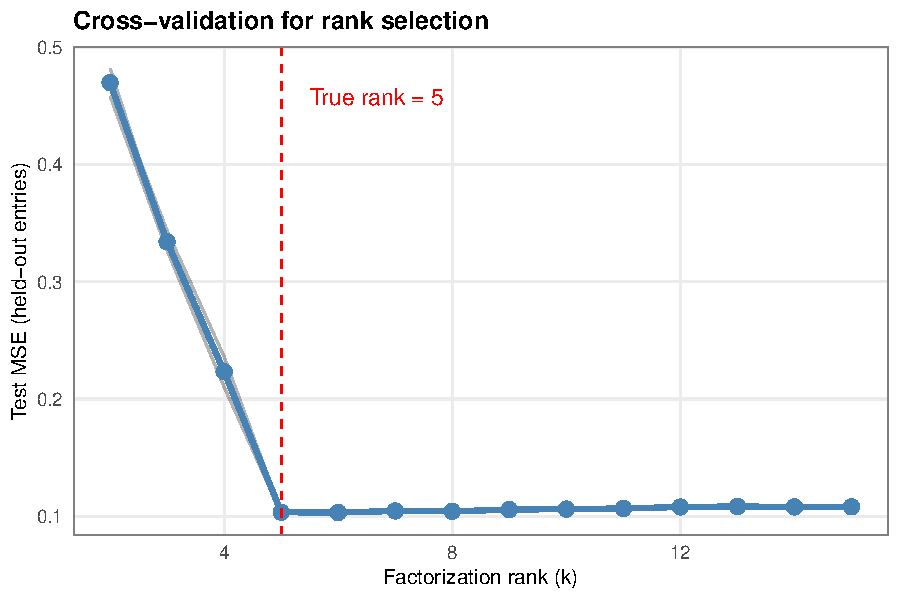
\includegraphics[width=0.8\textwidth]{fig_cv_rank}
\caption{\label{fig:cv}Cross-validation for rank selection on synthetic data 
with true rank 5. Test MSE is minimized near the true rank.}
\end{figure}

\subsection{Automatic rank determination}

For fully automated rank selection:

\begin{lstlisting}
R> model_auto <- nmf(A, k = "auto", cv_k_init = 2, cv_max_k = 20,
+    cv_tolerance = 2, maxit = 50, verbose = FALSE)
R> cat("Selected rank:", ncol(model_auto@w), "\n")
Selected rank: 10
\end{lstlisting}

\subsection{Regularization effects}

L1 regularization promotes sparsity in the factor matrices. Figure~\ref{fig:l1} 
shows the trade-off between reconstruction error and factor sparsity.

\begin{figure}[t]
\centering
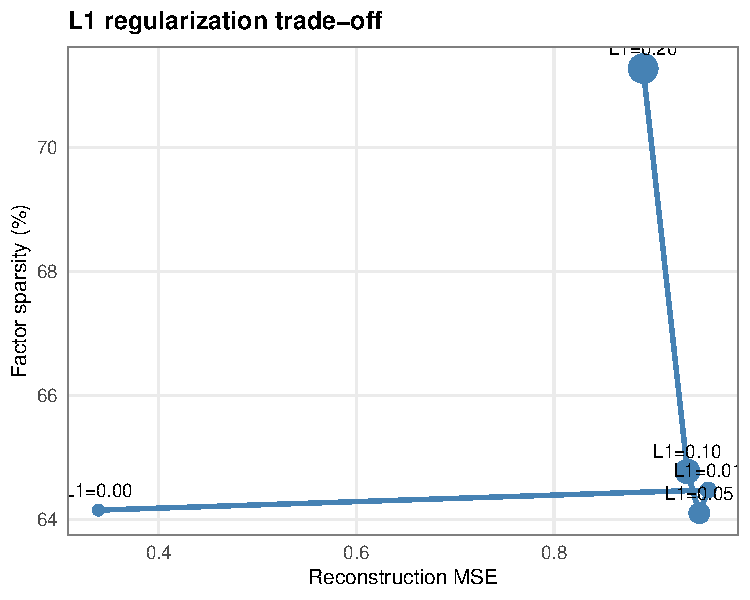
\includegraphics[width=0.7\textwidth]{fig_l1_tradeoff}
\caption{\label{fig:l1}L1 regularization trade-off between reconstruction 
error and factor sparsity.}
\end{figure}

\subsection{Scaling behavior}

Figure~\ref{fig:scaling} shows runtime scaling for sparse and dense matrices 
of increasing size.

\begin{figure}[t]
\centering
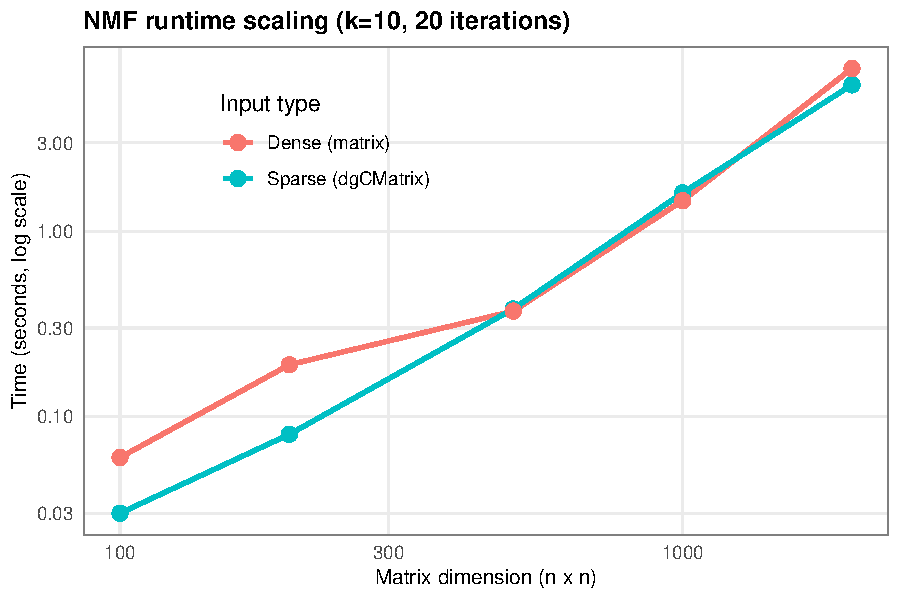
\includegraphics[width=0.8\textwidth]{fig_scaling}
\caption{\label{fig:scaling}Runtime scaling for NMF on sparse and dense 
matrices of increasing dimension.}
\end{figure}


%% =============================================================================
\section{Summary and discussion} \label{sec:summary}

The \pkg{RcppML} package provides a comprehensive NMF implementation for 
\proglang{R} with several distinguishing features. The integrated 
cross-validation framework enables principled rank selection with minimal 
overhead through streaming loss accumulation and position-dependent masking. 
Support for multiple loss functions via IRLS provides robustness to outliers 
common in real data. The automatic rank determination feature eliminates manual 
tuning through golden section search. Finally, the specialized rank-2 
implementation enables high-performance spectral bipartitioning competitive with 
truncated SVD.

The package achieves high performance through careful algorithm engineering: 
sequential coordinate descent with incremental residual updates, template 
metaprogramming for unified sparse/dense support, and cache-aware memory access 
patterns. Future work may explore parallel implementations for very large 
matrices and integration with GPU computing frameworks.

\pkg{RcppML} is available on CRAN and actively developed on GitHub. The 
header-only \proglang{C++} library can also be used directly for embedding in 
other applications.


%% =============================================================================
%% -- Computational details ----------------------------------------------------

\section*{Computational details}

The results in this paper were obtained using \proglang{R}~4.5.0 with the 
packages \pkg{RcppML}~1.0.0, \pkg{Matrix}~1.7.3, \pkg{irlba}~2.3.5.1, and 
\pkg{ggplot2}~4.0.1. \proglang{R} itself and all packages used are available 
from the Comprehensive \proglang{R} Archive Network (CRAN) at 
\url{https://CRAN.R-project.org/}.


%% -- Acknowledgments ----------------------------------------------------------

\section*{Acknowledgments}

The author thanks the \pkg{Rcpp} developers for the excellent \proglang{R} and 
\proglang{C++} integration framework.


%% -- Bibliography -------------------------------------------------------------

\bibliographystyle{plainnat}
\bibliography{refs}


%% -- Appendix -----------------------------------------------------------------

\appendix

\section{Algorithm pseudocode} \label{app:pseudocode}

Algorithm~\ref{alg:nmf_full} presents the complete NMF algorithm with 
cross-validation.

\begin{algorithm}[h]
\caption{NMF with cross-validation}
\label{alg:nmf_full}
\begin{algorithmic}[1]
\Require Matrix $\mathbf{A}$, rank $k$, CV fraction $p$, tolerance $\tau$, 
max iterations $T$
\State Initialize $\mathbf{W}$, $\mathbf{H}$, $\mathbf{D} = \mathbf{I}$
\State Generate mask seed
\For{$t = 1, \ldots, T$}
  \State // Update H
  \For{$j = 1, \ldots, n$}
    \State $\mathbf{a}_j^{\text{train}} \leftarrow \text{ApplyMask}(\mathbf{a}_j, j, p, \text{seed})$
    \State $\mathbf{h}_j, \mathbf{r}_j \leftarrow \text{NNLS}(\mathbf{a}_j^{\text{train}}, 
    \mathbf{WD}, \lambda_1)$
    \State $\text{test\_mse} \mathrel{+}= \text{MaskedSquaredResiduals}(\mathbf{r}_j + 
    (\mathbf{a}_j - \mathbf{a}_j^{\text{train}}), j, p, \text{seed})$
  \EndFor
  \State // Update W (similar, transposed)
  \State // Update scaling
  \For{$i = 1, \ldots, k$}
    \State $d_i \leftarrow d_i \cdot \|\mathbf{w}_i\|_2$
    \State $\mathbf{w}_i \leftarrow \mathbf{w}_i / \|\mathbf{w}_i\|_2$
  \EndFor
  \State // Check convergence
  \If{relative change in $\mathbf{W}$ and $\mathbf{H}$ $< \tau$}
    \State \textbf{break}
  \EndIf
\EndFor
\State \Return $\mathbf{W}$, $\mathbf{D}$, $\mathbf{H}$, test\_mse
\end{algorithmic}
\end{algorithm}

\section{IRLS weight derivations} \label{app:irls}

For each loss function $\rho(r)$, the IRLS weight is $w(r) = \rho'(r)/r$:

\paragraph{MAE.} $\rho(r) = |r|$, so $\rho'(r) = \text{sign}(r)$ and 
$w(r) = 1/|r|$.

\paragraph{Huber.} 
\[
\rho'(r) = \begin{cases} r & |r| \leq \delta \\ \delta \cdot \text{sign}(r) & 
|r| > \delta \end{cases}
\]
Thus $w(r) = \min(1, \delta/|r|)$.

\paragraph{KL-divergence.} For $\rho(a, \hat{a}) = a\log(a/\hat{a}) - a + 
\hat{a}$, taking derivative with respect to $\hat{a}$: $\partial\rho/
\partial\hat{a} = 1 - a/\hat{a}$. The weight is $w = a/\hat{a}^2$.

\end{document}
